\setcounter{rownumber}{0}
\singlespacing
\chapter{Manuscript I: Laser cooling of traveling wave phonons in an optical fiber}
\label{chap: 2-Cooling}
\acresetall

%  Copy this file for each main chapter, make sure to add it to main.tex

% Example author list with footnote style affiliations

Joel N. Johnson\footnote{\label{NAU}
Department of Applied Physics and Materials Science, Northern Arizona University, Flagstaff, AZ 86011, USA
}$^,$\footnote{\label{MIRA}
Center for Materials Interfaces in Research and Applications, Flagstaff, AZ 86011, USA
},
Danielle R. Haverkamp$^\mathrm{\ref{NAU}}$$^,$$^\mathrm{\ref{MIRA}}$,
Yi-Hsin Ou\footnote{\label{UofA}
College of Optical Sciences, University of Arizona, 1630 E University Blvd, Tucson, AZ 85721, USA
},
Khanh Kieu$^\mathrm{\ref{UofA}}$,
Nils T. Otterstrom\footnote{\label{Sandia}
Sandia National Laboratory, 1515 Eubank Blvd SE, Albuquerque, NM 87123, USA
},
Peter T. Rakich\footnote{\label{Yale}
Department of Applied Physics, Yale University, New Haven, CT 06520, USA
},
Ryan O. Behunin$^\mathrm{\ref{NAU}}$$^,$$^\mathrm{\ref{MIRA}}$

\hfill

%  Extra copyright disclaimer to be safe

\textit{This is the Accepted Manuscript version of an article accepted for publication in Physical Review Applied. Wiley Inc is not responsible for any errors or omissions in this version of the manuscript or any version derived from it. The Version of Record is available online at} \url{https://doi.org/}\textit{.}

\doublespacing

%%%%%%%%%%%%%%%%%%%%%%%%%%%%%%%%%%%%%%%%%%%%%%%%%%%%%%%%%%%%%%%%%%%%
%  Chapter contents here

\section{Abstract}
In recent years, optical control of mechanical oscillators has emerged as a critical tool for everything from information processing to laser cooling. While traditional forms of optomechanical cooling utilize systems comprising discrete optical and mechanical modes, it has recently been shown that cooling can be achieved in a chip-based system that possesses a continuum of modes. Through Brillouin-mediated phonon photon interactions, cooling of a band of traveling acoustic waves can occur when anti-Stokes scattered photons exit the system more rapidly than the relaxation rate of the mechanical waves, to a degree determined by the acousto-optic coupling. Here, we demonstrate that a continuum of travelingwave phonons can be cooled within an optical fiber, extending this physics to macroscopic length scales. Leveraging the large acousto-optic coupling permitted within a liquid-core optical fiber, heterodyne spectroscopy reveals power-dependent changes in spontaneous-Brillouin-scattering spectra that indicate a reduction of the thermal phonon population by 21 K using 120 mW of injected laser power. These results provide alternative ways to manipulate phonon populations that could enable acousto-optic applications Q2 with reduced noise or provide ways to control traveling-wave phonons at the quantum level.

\hfill

\section{Introduction}
Laser cooling has brought about a revolution in \ac{AMO} physics, permitting exquisite control of the motion of ions, atoms, and molecules, precision measurements of time, and the creation of alternative states of matter \citep{hansch1975cooling, ashkin1978trapping, wineland1978radiation, phillips1982laser, anderson1995observation, davis1995bose, ludlow2015optical, epstein1995observation, sheik2007optical}. Beyond these \ac{AMO} applications, laser cooling has led to impressive developments in solid-state systems where optical refrigeration in rare earth doped glasses is rapidly approaching cryogenic operation, and sideband cooling of individual mesoscopic mechanical oscillators has opened new windows to the foundations of physics and enabled the generation of novel quantum states \citep{chan2011laser, marshall2003towards, hong2017hanbury, aspelmeyer2014cavity}.

Laser cooling of mechanical oscillators conventionally utilize an optical cavity with a movable mirror where radiation pressure mediates a parametric coupling between cavity resonance and a discrete phononic mode \citep{aspelmeyer2014cavity}. This configuration is critical to optical sideband cooling, where drive laser photons, with frequencies red-detuned from an optical resonance, can preferentially blue-shift by phonon scattering, rapidly exit the system, and lower the effective phonon occupancy \citep{aspelmeyer2014cavity}. While optomechanical cooling of traveling wave phonons has been achieved in whispering gallery mode resonators that support discrete optical and mechanical modes \citep{bahl2012observation}, surprisingly, this form of anti-Stokes cooling can occur in continuous systems---without optical or mechanical resonances \citep{otterstrom2018optomechanical}. Otterstrom {\it et al.} showed that cooling of a continuous band of phonon modes can be achieved when injected laser light scatters through an anti-Stokes process from traveling wave phonons and exits the system more rapidly than the phonon bath returns to thermal equilibrium.  Because distinct traveling phonon modes mediate Stokes and anti-Stokes scattering in a continuous system, it is possible to cool a selected band of phonons as any simultaneous Stokes `heating' will change the population of a distinct mode. This form of cooling simultaneously requires substantial light-sound couplings, to enable efficient scattering, and phonon lifetimes exceeding the transit time for light through the waveguide. Owing to these stringent requirements, optomechanical cooling in continuous systems has only been observed in silicon waveguides engineered to have large Brillouin coupling and short $\sim$ cm lengths. While the realization of this physics within optical fibers may be attractive for low-noise signal processing, high-coherence lasers, high-fidelity optical squeezing, and variable bandwidth forms of all-optical slow-light generation, demonstration of cooling of travelling wave phonons in fibers has remained elusive \citep{shin2015control,shelby1986generation,okawachi2005tunable}.

Here, we demonstrate cooling of a continuum of phonon modes in optical fiber for the first time. Through spontaneous Brillouin scattering in a 1m long CS$_2$-filled liquid-core optical fiber, we achieve cooling (i.e., change in temperature) of $\sim$21K from room temperature for a band of anti-Stokes phonons. These dynamics are made possible by the unique features of this fiber system (Fig. \ref{fig:cooling-system})\citep{kieu2013brillouin,kieu2014nonlinear,behunin2019spontaneous}. The large refractive index and small sound speed of CS$_2$ enable simultaneous guidance and tight co-confinement of light and sound (Fig. \ref{fig:cooling-system}c \& d) within small diameter silica capillaries. This tight acousto-optic overlap, combined with the large electrostrictive coupling made possible within CS$_2$ \citep{boyd2020nonlinear} permit large light-sound interactions which can be leveraged for optomechanical cooling in a continuous system.

\begin{figure*}[t]
    \centering
    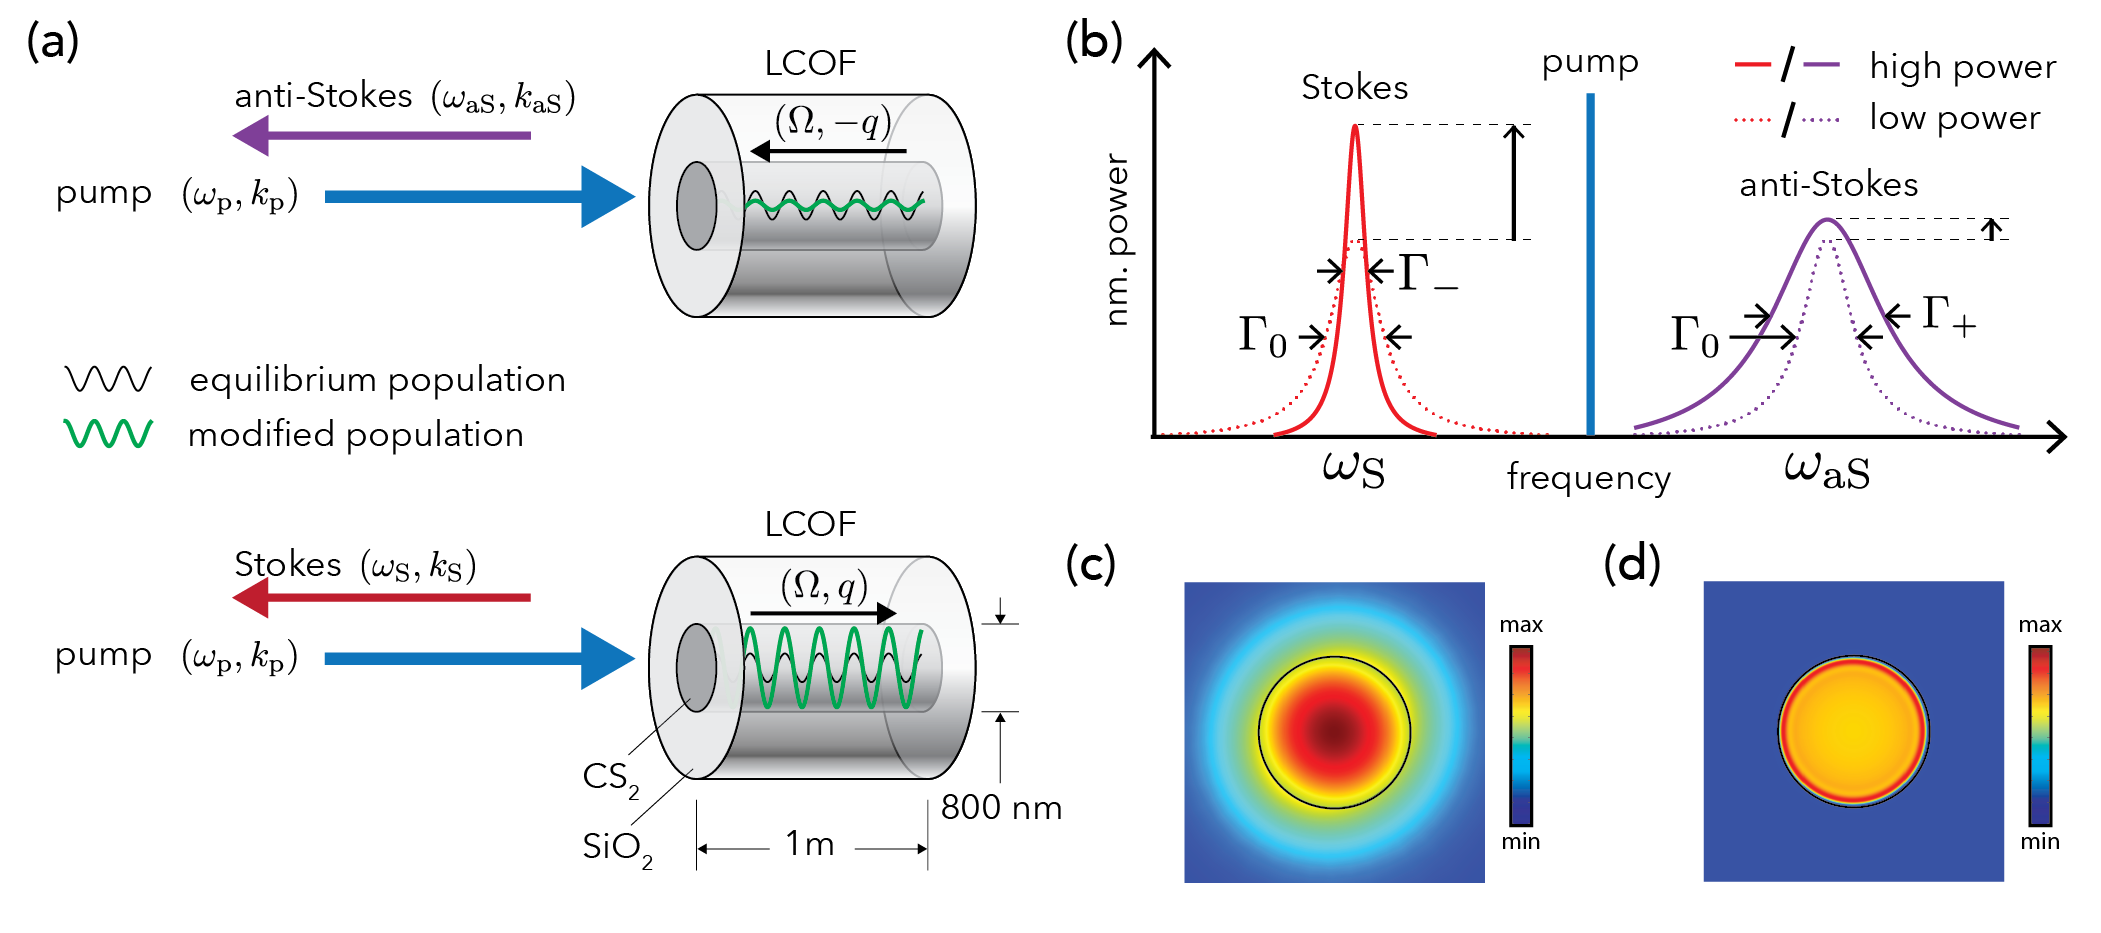
\includegraphics[width=\textwidth]{figs/2-Cooling/introFig_Cooling_v3-01.png}
    \caption{Illustration of (a) geometry and scattering processes in a \ac{LCOF}, (b) cooling signatures in spontaneous light scattering spectra, and simulated (c) optical and (d) mechanical modes. Simulations (c) and (d) plot the magnitudes of the electric and displacement fields respectively.}
    \label{fig:cooling-system}
\end{figure*}

Using heterodyne spectroscopy, we show how spontaneously scattered power spectra evolve with pump power. These spectra reveal the signatures of cooling, showing changes in the phonon dissipation rate and nonlinear dependence on the pump power. To confirm depletion of thermal phonons, we perform a form of pump-probe spontaneous Brillouin scattering where changes in the phonon population can be directly probed. This pump-probe technique leverages a unique property of Brillouin scattering, permitting two orthogonal polarizations of light to couple to the same band of phonons. Using this feature an intense pump can be used to cool the phonon modes while a weak probe laser in an orthogonal polarization, that can be isolated from the pump, measures the phonon population. With fixed probe powers, these results show that the power of anti-Stokes scattered probe light decreases as the pump power is increased, indicating that the thermal population of the anti-Stokes phonons has been reduced in a manner consistent with theory. With the long lengths and power-handling capabilities of optical fibers, combined with recent theoretical developments, these results may enable new low-noise fiber applications, ground state cooling of bands of traveling phonon modes, and new forms of quantum state synthesis \citep{zhu2022dynamic,behunin2022quantum}.

\begin{figure*}[t]
    \centering
    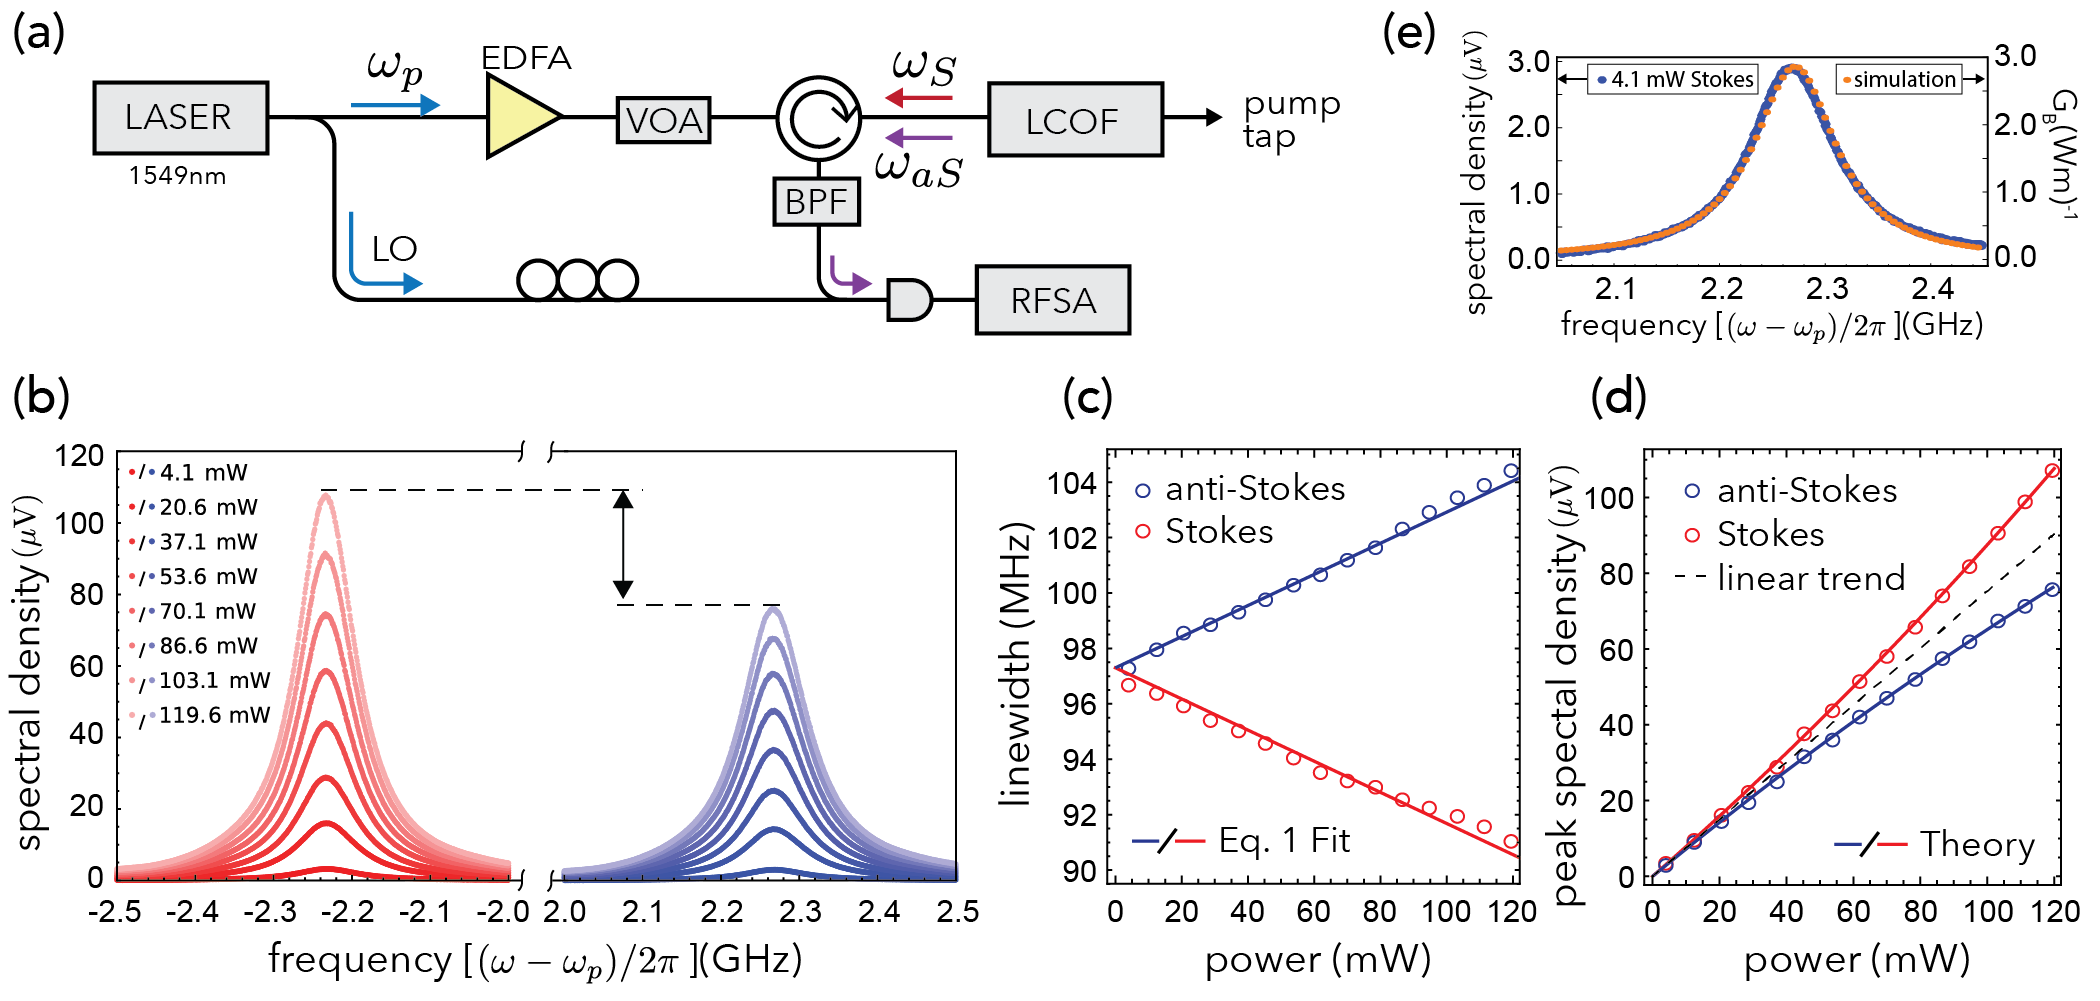
\includegraphics[width=\textwidth]{figs/2-Cooling/apparatus_pump_only_v3-01.png}
    \caption{(a) Heterodyne spectroscopy apparatus for measuring power dependence of spontaneous Brillouin spectra shown in (b). Lorentzian fits to spectra in (b) reveal signatures of Brillouin cooling through (c) power-dependent linewidths and (d) sub- and super-linear growth of the power spectra peaks. The lines in (c) are obtained through a constrained fit using Eq. \ref{eq:gamma} providing an estimated Brillouin gain of 2.3 (Wm)$^{-1}$. Theory in (d) obtained using the fitted value of $G_B$, Eq. \eqref{eq:neff} and the measured spectra heights at 4.1 mW (see Appendix A).(e) Comparison between measured and simulated light scattering spectra (see Appendix C). Here, EDFA stands for Erbium doped fiber amplifier, BPF is a tunable band-pass filter, and VOA is variable optical attenuator.}
    \label{fig:cooling-results-1}
\end{figure*}

\section{Laser cooling of traveling wave phonons}
Laser cooling of traveling wave phonons occurs through anti-Stokes Brillouin scattering. During this process an incident pump photon annihilates a counter-propagating phonon, blue-shifts to higher energy, and rapidly exits the system (Fig. \ref{fig:cooling-system}a).
%
The frequencies and wavevectors of the participating guided waves satisfy the following phase-matching conditions
\begin{align}
\label{pm-1}
    &\omega_p + \Omega = \omega_{aS} \\
    \label{pm-2}
    &k_p - q = -k_{as}
\end{align}
where the angular frequencies (wavevectors) for the pump, phonon, and anti-Stokes modes are given by $\omega_p$, $\Omega$, and $\omega_{aS}$ ($k_p$, $-q$, and $-k_{aS}$). Here, the propagation direction of the mode is denoted by the sign of the wavevector. For a selected pump frequency, the dispersion relations, for both light and mechanical waves, and Eqs. \eqref{pm-1}\& \eqref{pm-2} can be used to find the frequency of the traveling wave phonon that participates in anti-Stokes Brillouin scattering
\begin{align}
\label{pm-3}
    \Omega \approx \frac{2 n v}{c}\omega_p
\end{align}
where $n$ is the refractive index, $v$ is the speed of sound, and $c$ is the speed of light in vacuum. It is important to note that Stokes scattering will also occur within the system, tending to increase the population of phased-matched phonons that co-propagate with the pump (Fig. \ref{fig:cooling-system} a). As a result, `heating' of the phonons participating in the Stokes process and cooling of the distinct counter-propagating phonon mode mediating anti-Stokes scattering will proceed simultaneously. While cooling of a band of traveling wave phonons can be achieved and independently detected, unless Stokes scattering is suppressed, the system as a whole will not be cooled.

In order for cooling to occur, the mechanical degrees of freedom must return to thermal equilibrium more slowly than the anti-Stokes photons exit the system. A mean-field analysis of these dynamics, described in Appendix A, shows that these conditions require $4v_g/L > \Gamma_0$, where $v_g$ is the optical group velocity, $L$ is the system length and $\Gamma_0$ is the mechanical dissipation rate \citep{otterstrom2018optomechanical}, conditions met by the system considered here (Fig. \ref{fig:cooling-system}(a)) with $4 v_g/L \approx 0.82$ GHz and $\Gamma_0 \approx 0.61$ GHz. While these disparate optical and mechanical timescales allow the phonon population to be driven out of thermal equilibrium, the degree of cooling requires a relatively large single pass Brillouin gain $G \equiv G_B P_p L$ where $G_B$ is the Brillouin gain coefficient [m$^{-1}$W$^{-1}$] and $P_p$ is the pump power \citep{boyd2020nonlinear}, yielding a fractional temperature $\Delta T/T_0$ change given approximately by
\begin{equation}
\label{eq:FFC}
   \frac{\Delta T}{T_0} \approx \frac{G}{G+4}
\end{equation}
where $T_0$ is the equilibrium temperature \citep{otterstrom2018optomechanical}. Therefore, we must balance competing requirements, maximizing the single-pass gain while minimizing the light travel time across the fiber to achieve efficient cooling. Although the mean-field optical decay rate is marginally greater than the phonon decay rate, analysis of the coupled envelope dynamics shows that the key conclusions of the mean-field analysis remain valid in the limit of small single-pass gains explored here (see Appendix A.1).

Cooling of traveling wave phonons can be identified by power-dependent changes in the width and height of spontaneous light scattering spectra, revealing the phonon band temperature and dissipation rate (Fig. \ref{fig:cooling-system}b). While for low power ($G \ll 1$) the spectrum height increases linearly with pump power, these increases begin to saturate (grow more rapidly) for the anti-Stokes (Stokes) spectrum as the single pass gain approaches one and the phonon population is depleted (increased). Consequently, the anti-Stokes (Stokes) spectrum height grows sub-linearly (super-linearly), depending on both the pump power and the phonon population (Figs. \ref{fig:cooling-system}b \& \ref{fig:cooling-results-1}d). Owing to additional decay (amplification) channels opened by spontaneous anti-Stokes (Stokes) Brillouin scattering, the phonon dissipation rate increases (decreases) with pump power according to
\begin{equation}
\label{eq:gamma}
   \Gamma_{\pm} \approx \Gamma_0\left(1\pm \frac{1}{4}G\right)
\end{equation}
where the upper (+) sign indicates an increase in the anti-Stokes phonon decay rate and the lower (-) sign quantifies how the Stokes spectrum narrows \citep{otterstrom2018optomechanical}.
%
Interestingly, the Brillouin nonlinearity increases the group velocity of the anti-Stokes photons  \citep{gonzalez2005optically}. As a result, the conditions for cooling can be met even as the phonon decay rate increases, i.e., $4 v_{g,eff}/L > \Gamma_+$ (see Appendix Sec. A)
%
As a consequence of these altered decay rates, detailed balance for thermal equilibrium is broken, reducing (or increasing) the effective population of the anti-Stokes (Stokes) phonons $n^+_{eff}$($n^-_{eff}$) described by
\begin{equation}
\label{eq:neff}
    n^{\pm}_{eff} \approx \frac{\Gamma_0}{\Gamma_{\pm}} n_{th},
\end{equation}
where $n_{th} \approx 2700$, given by the Bose distribution, is the occupation number for the relevant phonons in our \acf{LCOF} in thermal equilibrium \citep{otterstrom2018optomechanical}. See Appendix A for more details of the mean-field analysis of the nonlinear optics in this system.

To demonstrate this physics, we utilize a 1m long CS$_2$-filled silica capillary (Fig. \ref{fig:cooling-system}), possessing an array of properties that are ideal for laser cooling of traveling wave phonons. The materials properties and geometry of this liquid-filled capillary permit guided optical (single-mode at 1.55 $\mu$m) (Fig. \ref{fig:cooling-system}c) and acoustic waves (Fig. \ref{fig:cooling-system}d) within the $800$nm diameter fiber core and enable large Brillouin gain (see Tab. I in App. C for more details). Furthermore, macroscopic meter-scale lengths make large single-pass gain accessible at modest sub-Watt powers. See Refs. \citep{kieu2013brillouin,kieu2014nonlinear,behunin2019spontaneous} for details on Brillouin scattering in \ac{LCOF}s.

\section{Methods \& Results}
We measure Brillouin cooling in this \ac{LCOF} using the apparatus shown in Fig. \ref{fig:cooling-results-1}a. The output of a laser is split in two, a variable power arm is injected into the sample for Brillouin cooling, and a fixed-power arm is used to synthesize a \ac{LO} for heterodyne detection. Spontaneously backscattered light is filtered, to remove stray pump light and isolate the anti-Stokes (or Stokes) sideband, photomixed with the \ac{LO} on a high-speed receiver, and detected on a \ac{RFSA} as a function of pump power. These measurements yield spontaneous Brillouin scattering spectra of the type shown in Fig. \ref{fig:cooling-results-1}b.

\begin{figure*}[t]
    \centering 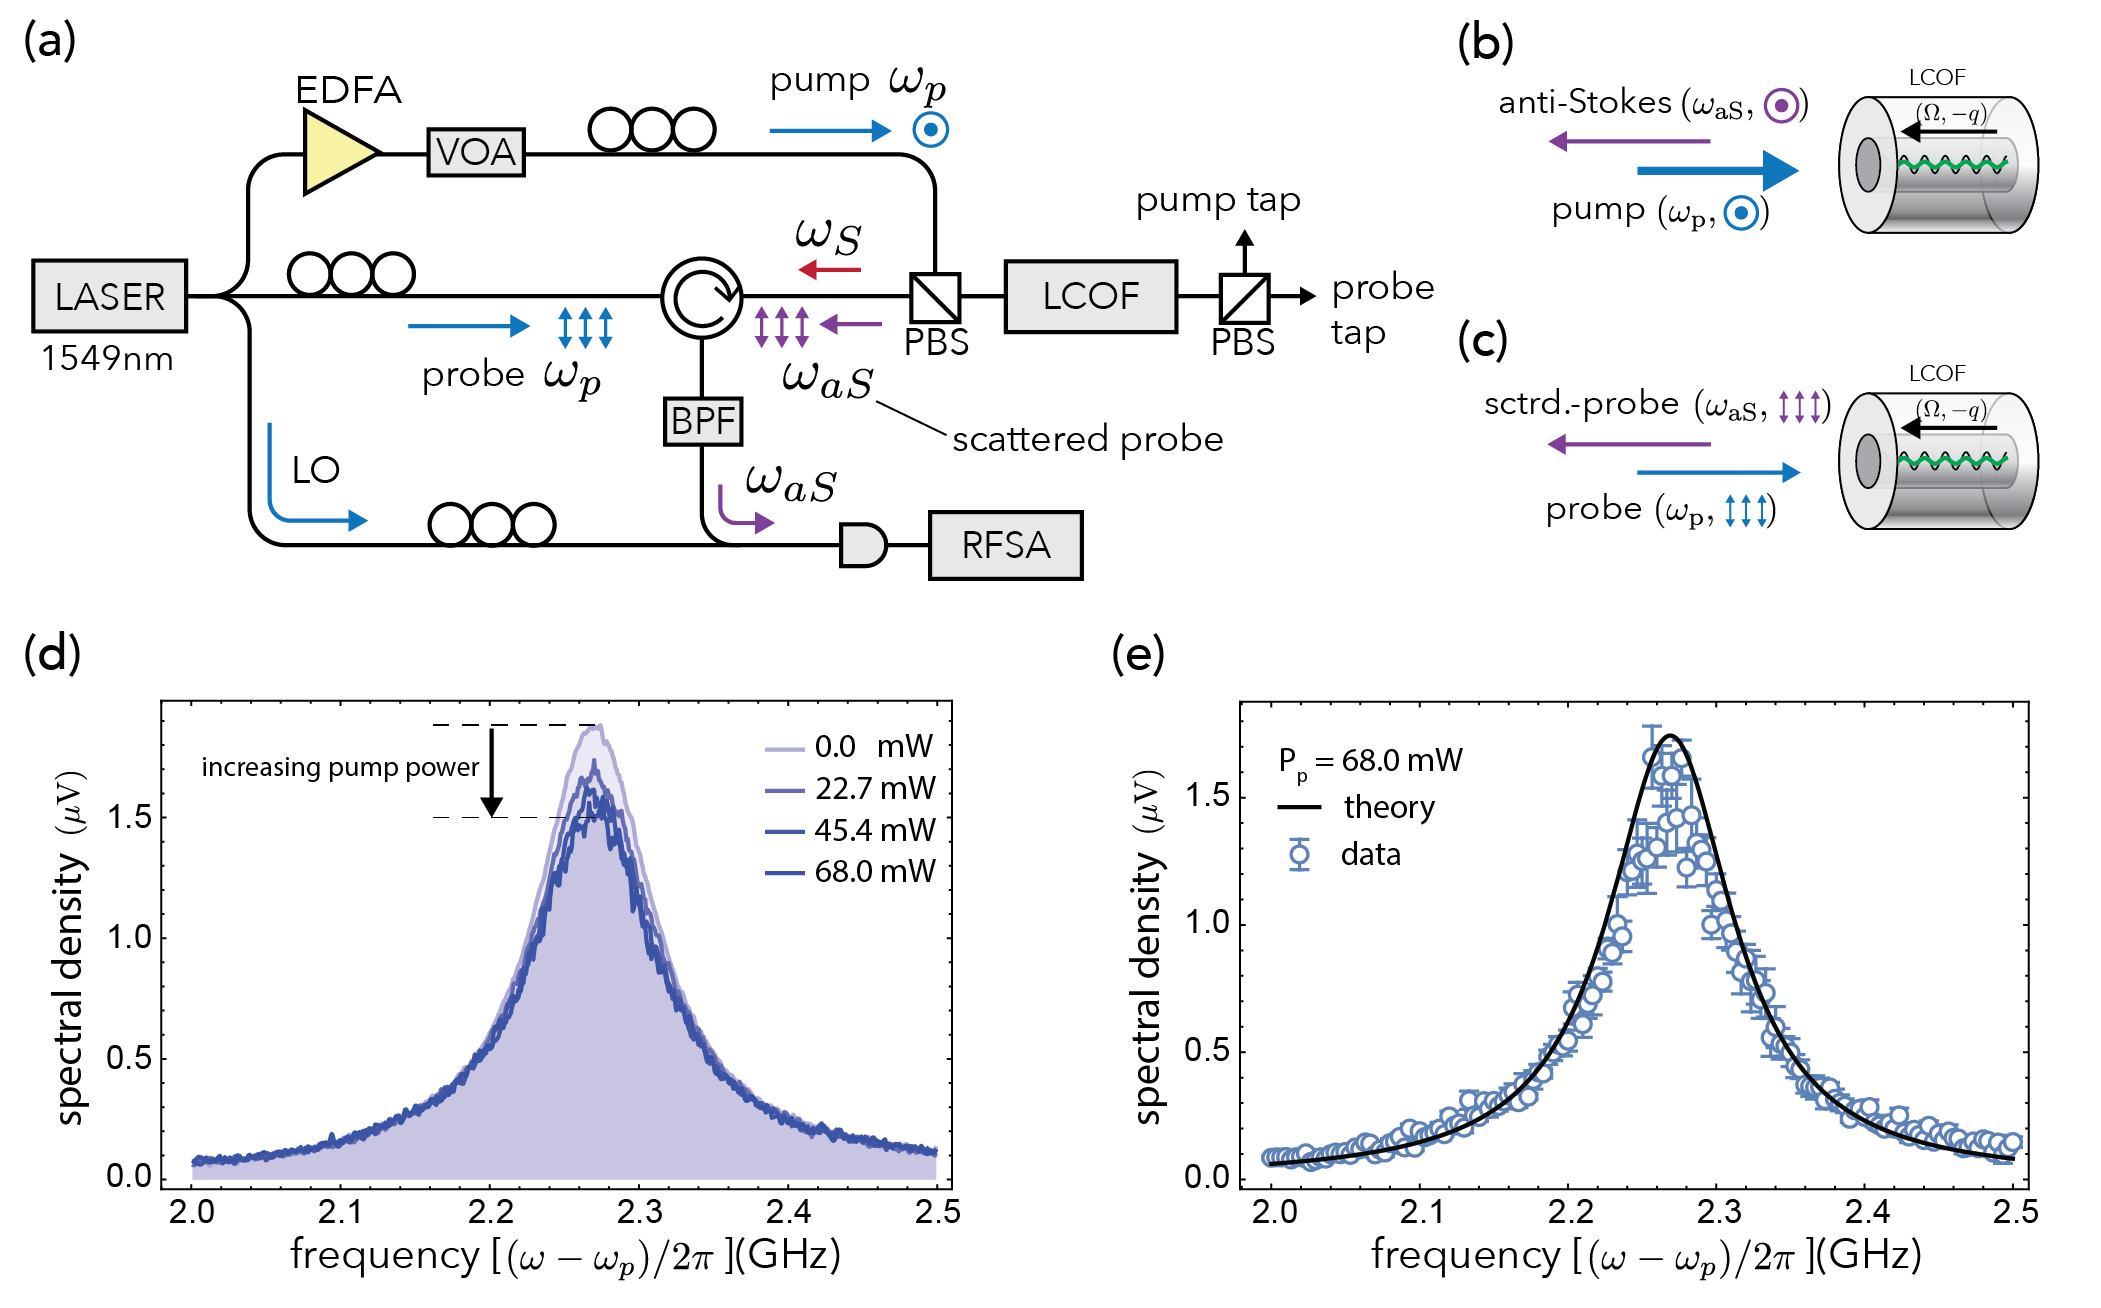
\includegraphics[width=0.95\textwidth]{figs/2-Cooling/apparatus_pump_probe_v4-01.png}
    \caption{Pump-probe measurements of Brillouin cooling. (a) Pump-probe spectrometer. Orthogonally polarized pump and fixed-power probe light are combined and sent into the sample using a \ac{PBS}. Backscattered pump and probe light exit distinct ports of the PBS, and anti-Stokes sideband is isolated using a circulator and tunable  \ac{BPF}. Orthogonally polarized pump and probe beams (b) and (c) couple to the same band of phonons. The scattered probe can be isolated from the scattered pump using a PBS.
    (d) Backscattered anti-Stokes power spectra for the probe plotted for various pump powers. For clarity the data is averaged over 1.67 MHz bins. (e) Comparison of measured anti-Stokes spectra and the power spectrum predicted by mean-field theory (see Appendix B).}
    \label{fig:cooling-results-2}
\end{figure*}

The data displayed in Fig. \ref{fig:cooling-results-1} exhibit key signatures of Brillouin cooling. With increasing pump power, the linewidth of the anti-Stokes spectrum increases and the scattered anti-Stokes power increases sub-linearly (Fig. \ref{fig:cooling-results-1}c \& d). The extracted linewidths of the Stokes and anti-Stokes spectra exhibit the power dependence described by Eq. \eqref{eq:gamma}, yielding a Brillouin gain coefficient $G_B \sim 2.3$(Wm)$^{-1}$, qualitatively described by finite-element simulations shown in Fig. \ref{fig:cooling-results-1}e predicting $G_B \approx 2.9$ (Wm)$^{-1}$. %The discrepancy in measured and simulated Brillouin gain can be explained as a consequence of the inherent uncertainties in the intra-fiber power, quantified by the coupling losses through the entrance splice which cannot be measured independently.
Using Eq. \eqref{eq:FFC}, these measurements show that the temperature of the band of traveling anti-Stokes phonons has been reduced by 21K from room temperature for 120mW of pump power.

The apparatus and data shown in Fig. \ref{fig:cooling-results-1} directly demonstrate the signatures of laser cooling of a continuous band of phonons. However, in these measurements, the amplitude of the power spectrum is proportional to the product of phonon population and the pump power. To directly detect changes to the phonon population, we utilize a form of pump-probe spectroscopy shown in Fig. \ref{fig:cooling-results-2}. In contrast with the heterodyne measurements depicted in Fig. \ref{fig:cooling-results-1}, the output of a laser is divided into a variable power pump, and a fixed power probe. Orthogonally polarized pump and probe beams are combined using a \acf{PBS} and sent into the \ac{LCOF} where they interact with the same phonon mode (Fig. \ref{fig:cooling-results-2} b \& c). Owing to this polarization multiplexing, spontaneously back-scattered probe light is separated from the backscattered pump by the \ac{PBS}, filtered, and photomixed with the \ac{LO} for heterodyne detection, yielding the spectra shown in Fig. \ref{fig:cooling-results-2}d. Consistent with the depopulation of phonons, these results show a decrease in the anti-Stokes scattering rate with increasing in pump power. Furthermore, Fig. \ref{fig:cooling-results-2}c shows that these spectra are well-described by a simple model of the pump-probe dynamics with parameters obtained from independent measurements shown in Fig. \ref{fig:cooling-results-1}. See Appendix B for further details of the pump-probe theory.

\section{Conclusions}
We have demonstrated laser cooling of travelling wave phonons in an optical fiber for the first time.  Using spontaneous Brillouin light scattering spectroscopy of a CS$_2$-filled \ac{LCOF}, we probe the populations of travelling wave phonons, revealing power-dependent changes in the phonon dynamics consistent with a mean-field model and finite-element simulations. Key to accessing this regime of light matter interactions is the large acousto-optic coupling and short length of our sample, where pump photons readily scatter from counter-propagating phonons and rapidly exit the fiber before the phonons can return to thermal equilibrium. The combination of these properties enables 21K of phonon cooling for 120mW of pump power.

Building on these results, drastic enhancements in our ability to cool traveling wave phonons may be achievable with changes in the fiber geometry and material. With larger core diameters, the Brillouin gain can be dramatically increased through improved acousto-optic overlap as well as through increased optical intensity. Working toward the limit of single-mode operation (for 1.55 $\mu$m optical wavelengths), finite-element simulations predict Brillouin gains of $\sim$ 11 (Wm)$^{-1}$ for a \ac{LCOF} with a 1.6 $\mu$m core diameter, exceeding the acousto-optic coupling in our \ac{LCOF} by nearly a factor of five. Under the same experimental conditions as this study, such a fiber could achieve 119 K of cooling for 250 mW of pump power, approaching cryogenic temperatures. Alternatively, chalcogenide glass fibers can be used to achieve much large Brillouin gains \citep{abedin2005observation}. For example, $6 \mu$m core diameter As$_2$Se$_3$ fibers achieve bulk Brillouin gain of $g_B = 6.2 \times 10^{-9}$ m/W, translating to an approximate Brillouin gain coefficient of  $G_B \sim 159$ (Wm)$^{-1}$. In such a system, Eq. \eqref{eq:FFC} shows that 100K of cooling can be achieved in a 1 m fiber with 13mW of pump power.

As thermal noise produced by traveling wave phonons is a critical limitation in a variety of fiber-based applications including information processing, lasers, and quantum optics experiments, these results may inspire new ways to achieve improved performance.  The techniques demonstrated in this paper may be used to create new Brillouin laser technologies with superb stability \citep{behunin2018fundamental,li2012characterization}, reduce backscatter produced by spontaneous Brillouin scattering in fiber optic communications, suppress guided acoustic wave modulation of quantum optical signals, or enable all-optical delay lines with tunable bandwidth \citep{okawachi2005tunable}.

\section{Acknowledgements}

J. J. and R. B. acknowledge funding from NSF Award No. 2145724. This article has been authored by an employee of National Technology \& Engineering Solutions of Sandia, LLC under Contract No. DE-NA0003525 with the U.S. Department of Energy (DOE). The employee owns all right, title and interest in and to the article and is solely responsible for its contents. The United States Government retains and the publisher, by accepting the article for publication, acknowledges that the United States Government retains a non-exclusive, paid-up, irrevocable, world-wide license to publish or reproduce the published form of this article or allow others to do so, for United States Government purposes. The DOE will provide public access to these results of federally sponsored research in accordance with the DOE Public Access Plan \url{https://www.energy.gov/downloads/doe-public-access-plan}.
